\documentclass{beamer}
\usepackage{alltt}
\usepackage{tikz}
\usetikzlibrary{matrix}
\usetikzlibrary{trees}
\usepackage{cancel}
\usepackage{subcaption}
\PassOptionsToPackage{obeyspaces}{url}
\usepackage{hyperref}
\usepackage{adjustbox}

\usepackage{lipsum}

\usetheme{Hannover}

\newcommand{\racket}{\texttt{Racket}}
\newcommand{\drr}{\texttt{DrRacket}}
\newcommand{\fsm}{\texttt{FSM}}
\newcommand{\ide}{\texttt{IDE}}
\newcommand{\api}{\texttt{API}}
\newcommand{\arrow}{\(\rightarrow\)}
\newcommand{\dotss}{\(\ldots\)}
\newcommand{\vdotss}{\(\vdots\)}
\newcommand{\elist}{\texttt{\textquotesingle{()}}}
\newcommand{\logand}{\texttt{\(\wedge\)}}
\newcommand{\logor}{\texttt{\(\vee\)}}
\newcommand{\imp}{\texttt{\(\Rightarrow\)}}
\newcommand{\sig}{\texttt{\(\Sigma\)}}
\newcommand{\delt}{\texttt{\(\delta\)}}
\newcommand{\sigsig}{\texttt{\(\Sigma\) = \{a b\}}}
\newcommand{\gam}{\texttt{\(\Gamma\)}}
\newcommand{\ep}{\texttt{\(\epsilon\)}}
\newcommand{\quot}{\texttt{\textquotesingle{}}}
\newcommand{\dquot}{\texttt{"}}
\newcommand{\qquot}{\texttt{\textasciigrave{}}}
\newcommand{\lambexpr}{\texttt{$\lambda$}-expression}
\newcommand{\lamb}{\texttt{$\lambda$}}
\newcommand{\is}{\texttt{::=}}

\definecolor{darkgreen}{RGB}{102,170,102}

\begin{document}

\title{Part III: Expressions}
%\subtitle{Using Beamer}
\author{Marco T. Moraz\'{a}n}
\institute{Seton Hall University}
\date{}

\begin{frame}
\titlepage
\end{frame}

\begin{frame}
\frametitle{Outline}
\tableofcontents
\end{frame}

\section{A Language Based on an Extended Lambda Calculus}

\begin{frame}[fragile]
\frametitle{Automatic Parsing}
%\framesubtitle{HOMEWORK}
\begin{scriptsize}
\begin{itemize}
\item<1-> We will now study the semantics (or meaning) of some fundamental programming languages features

\item<1-> Our primary tools will be interpreters

\item<2->
\begin{center}
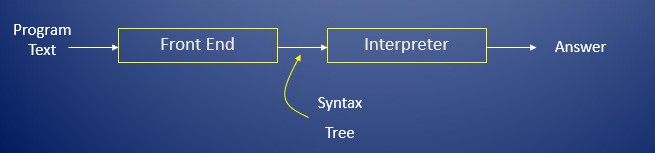
\includegraphics[scale=0.8]{interpreter-arch.jpg}
\end{center}

\end{itemize}
\end{scriptsize}
\end{frame}

\begin{frame}[fragile]
\frametitle{Automatic Parsing}
%\framesubtitle{HOMEWORK}
\begin{scriptsize}
\begin{itemize}
\item<1-> Adapted and Extended Lambda Calculus
\begin{tabular}{lll}
  $<$exp$>$ & \is{} & $<$number$>$ \\
            & \is{} & true \\
            & \is{} & false \\
            & \is{} & $<$id$>$ \\
            & \is{} & -($<$exp$>$, $<$exp$>$)\\
            & \is{} & zero?($<$exp$>$)\\
            & \is{} & if $<$exp$>$ then $<$exp$>$ else $<$exp$>$\\
            & \is{} & let \{$<$id$>$ = $<$exp$>$\}$^*$ in $<$exp$>$\\
            & \is{} & proc($<$id$>^*$) $<$exp$>$ \\
            & \is{} & ($<$exp$>$ $<$exp$>^*$) \\
            & \is{} & letrec \{identifier ($<$id$>^*$) = $<$exp$>$\}$^*$ in $<$exp$>$
    %\hline
\end{tabular}

\item<2-> We will use a parser generator system: sllgen

\item<2-> Read: Appendix  B

\end{itemize}
\end{scriptsize}
\end{frame}

\begin{frame}[fragile]
\frametitle{Automatic Parsing}
%\framesubtitle{HOMEWORK}
\begin{scriptsize}
\begin{itemize}
\item<1-> Boilerplate Code
\begin{alltt}
#lang eopl

(require rackunit "../eopl-extras.rkt")

;;;;;;;;;;;;;;;; grammatical specification ;;;;;;;;;;;;;;;;

(define the-lexical-spec
  \quot{}((whitespace (whitespace) skip)
    (comment ("\%" (arbno (not \(\textbackslash\)newline))) skip)
    (identifier
      (letter (arbno (or letter digit "_" "-" "?"))) symbol)
    (number (digit (arbno digit)) number)
    (number ("-" digit (arbno digit)) number)))
\end{alltt}

\end{itemize}
\end{scriptsize}
\end{frame}

\begin{frame}[fragile]
\frametitle{Automatic Parsing}
%\framesubtitle{HOMEWORK}
\begin{scriptsize}
\begin{itemize}
\item<1-> The Grammar (not boilerplate)
\begin{alltt}
\quot{}((program (expression) a-program)
\end{alltt}

\item<2->
\begin{alltt}
  (expression (number) const-exp)
  (expression ("true") true-exp)
  (expression ("false") false-exp)
  (expression (identifier) var-exp)
  \end{alltt}

\item<3->
\begin{alltt}
  (expression("-" "(" expression "," expression ")")diff-exp)
\end{alltt}

\item<4->
\begin{alltt}
  (expression ("zero?" "(" expression ")") zero?-exp)
\end{alltt}

\item<5->
\begin{alltt}
  (expression
    ("if" expression "then" expression "else" expression) if-exp)
\end{alltt}

\item<6->
\begin{alltt}
  (expression
    ("let"(arbno identifier"="expression)"in" expression) let-exp)
\end{alltt}

\item<7->
\begin{alltt}
  (expression
    ("proc" "(" (arbno identifier) ")" expression) proc-exp)
\end{alltt}

\item<8->
\begin{alltt}
  (expression ("(" expression (arbno expression) ")") call-exp)))
\end{alltt}

\item<9->
\begin{alltt}
(expression
  ("letrec"(arbno identifier"("(arbno identifier)")""="expression)
   "in" expression) letrec-exp)
\end{alltt}

\end{itemize}
\end{scriptsize}
\end{frame}

\begin{frame}[fragile]
\frametitle{Automatic Parsing}
%\framesubtitle{HOMEWORK}
\begin{scriptsize}
\begin{itemize}
\item<1-> Boilerplate
\begin{alltt}
(sllgen:make-define-datatypes the-lexical-spec the-grammar)

(define show-the-datatypes
  (lambda ()
    (sllgen:list-define-datatypes the-lexical-spec the-grammar)))

(define scan&parse
  (sllgen:make-string-parser the-lexical-spec the-grammar))

(define just-scan
  (sllgen:make-string-scanner the-lexical-spec the-grammar))
\end{alltt}

\end{itemize}
\end{scriptsize}
\end{frame}

\begin{frame}[fragile]
\frametitle{Automatic Parsing}
%\framesubtitle{HOMEWORK}
\begin{tiny}
\begin{itemize}
\item<1->
\begin{alltt}
> (show-the-datatypes)
((define-datatype program program? (a-program (a-program21 expression?)))
 (define-datatype
  expression
  expression?
  (const-exp (const-exp22 number?))
  (true-exp)
  (false-exp)
  (var-exp (var-exp23 symbol?))
  (diff-exp (diff-exp24 expression?) (diff-exp25 expression?))
  (zero?-exp (zero?-exp26 expression?))
  (if-exp (if-exp27 expression?) (if-exp28 expression?) (if-exp29 expression?))
  (let-exp
   (let-exp30 (list-of symbol?))
   (let-exp31 (list-of expression?))
   (let-exp32 expression?))
  (letrec-exp
   (letrec-exp33 (list-of symbol?))
   (letrec-exp34 (list-of (list-of symbol?)))
   (letrec-exp35 (list-of expression?))
   (letrec-exp36 expression?))
  (proc-exp (proc-exp37 (list-of symbol?)) (proc-exp38 expression?))
  (call-exp (call-exp39 expression?) (call-exp40 (list-of expression?)))))
\end{alltt}

\item<2->
\begin{alltt}
> (scan&parse "if 0 then 1 else 2")
#(struct:a-program
  #(struct:if-exp #(struct:const-exp 0) #(struct:const-exp 1) #(struct:const-exp 2)))
\end{alltt}

\end{itemize}
\end{tiny}
\end{frame}

\section{Evaluation Wrapper Functions and Tests}

\begin{frame}[fragile]
\frametitle{Evaluation Wrapper Functions and Tests}
%\framesubtitle{HOMEWORK}
\begin{scriptsize}
\begin{itemize}
\item<1->
\begin{alltt}
;; string \arrow{} a-program
;; Purpose: Parse the given extended LC-program
(define (parse p) (scan&parse p))
\end{alltt}

\item<2->
\begin{alltt}
;; string \arrow{} expval
;; Purpose: Evaluate the given extended LC-program
(define (eval string)
  (value-of-program (parse string)))
\end{alltt}

\end{itemize}
\end{scriptsize}
\end{frame}

\begin{frame}[fragile]
\frametitle{Evaluation Wrapper Functions and Tests}
%\framesubtitle{HOMEWORK}
\begin{tiny}
\begin{itemize}
\item<1->
\begin{alltt}
(check-equal? (eval "if zero?(1) then 1 else 2") (num-val 2))
(check-equal? (eval "-(15, 10)") (num-val 5))
(check-equal?
 (eval "let x = 10 in if zero?(-(x, x)) then x else 2")
 (num-val 10))
(check-equal? (eval "let decr = proc (a) -(a, 1) in (decr 30)")
              (num-val 29))
(check-equal? (eval "( proc (g) (g 30) proc (y) -(y, 1))")
              (num-val 29))
(check-equal? (eval "let x = 200
                     in let f = proc (z) -(z, x)
                        in let x = 100
                           in let g = proc (z) -(z, x)
                              in -((f 1), (g 1))")
              (num-val -100))
(check-equal? (eval "let sum = proc (x) proc (y) -(x, -(0, y)) in ((sum 3) 4)")
              (num-val 7))
(check-equal? (eval "let sum = proc (x) proc (y) -(x, -(0, y))
                     in letrec sigma (n) = if zero?(n)
                                           then 0
                                           else ((sum n) (sigma -(n, 1)))
                        in (sigma 5)")
              (num-val 15))
(check-equal? (eval "letrec even(n) = if zero?(n)
                                      then zero?(n)
                                      else if zero?(-(n, 1))
                                           then zero?(n)
                                           else (even -(n, 2))
                     in (even 501)")
              (bool-val #f))
\end{alltt}

\end{itemize}
\end{tiny}
\end{frame}


\section{Expressed and Denoted Values}

\begin{frame}[fragile]
\frametitle{Expressed and Denoted Values}
%\framesubtitle{HOMEWORK}
\begin{scriptsize}
\begin{itemize}
\item<1-> An important part of the specification of any programming language is the set of values the language manipulates

\item<2-> Each language has at least two sets:
  \begin{description}
    \item[Expressed values] Possible values of expressions
    \item[Denoted values] Values bound to variables
  \end{description}

\item<3-> In our extended $\lambda$-calculus
 \begin{itemize}
   \item Expressed values: Int, Bool, and Proc
   \item Denoted values: Int, Bool, Proc
 \end{itemize}

\item<4-> We need an interface for expressed values
  \begin{description}
    \item[Constructors]
      \begin{itemize}
        \item num-val: int \arrow{} expval
        \item bool-val: Boolean \arrow{} expval
        \item proc-val: (listof symbol) expression env \arrow{} expval
      \end{itemize}
    \item[Observers]
      \begin{itemize}
        \item expval-$>$int : expval \arrow{} int
        \item expval-$>$bool : expval \arrow{} boolean
        \item expval-$>$proc : expval \arrow{} proc
      \end{itemize}
  \end{description}

\end{itemize}
\end{scriptsize}
\end{frame}

\begin{frame}[fragile]
\frametitle{Expressed and Denoted Values}
%\framesubtitle{HOMEWORK}
\begin{tiny}
\begin{itemize}
\item<1-> Expressed values
\begin{alltt}
(define-datatype expval expval?
  (num-val (value number?))
  (bool-val (boolean boolean?))
  (proc-val (proc proc?)))
\end{alltt}

\item<2-> Extractors
\begin{alltt}
;; expval \arrow{} Int throws error
;; Purpose: Extract number from given expval
(define (expval2num v)
  (cases expval v
    (num-val (num) num)
    (else (expval-extractor-error \quot{}num-val v))))
\end{alltt}

\item<3->
\begin{alltt}
;; expval \arrow{} Bool throws error
;; Purpose: Extract Boolean from given expval
(define (expval2bool v)
  (cases expval v
    (bool-val (bool) bool)
    (else (expval-extractor-error \quot{}bool-val v))))
\end{alltt}

\item<4->
\begin{alltt}
;; expval \arrow{} proc throws error
;; Purpose: Extract proc from given expval
(define (expval2proc v)
  (cases expval v
    (proc-val (proc) proc)
    (else (expval-extractor-error \quot{}proc-val v))))
\end{alltt}

\item<5->
\begin{alltt}
;; symbol expval \arrow{} throws error
;; Purpose: Throw expval extraction error
(define (expval-extractor-error variant value)
  (eopl:error \quot{}expval-extractors "Looking for a ~s, given ~s"
              variant value))
\end{alltt}

\end{itemize}
\end{tiny}
\end{frame}

\section{Environment Datatype}

\begin{frame}[fragile]
\frametitle{Environment}
%\framesubtitle{HOMEWORK}
\begin{scriptsize}
\begin{itemize}
\item<1-> Having vars \arrow{} need for an environment

\item<1-> Discussed earlier in this course

\item<2-> Notation
 \begin{itemize}
	\item $[x=3] [y=7] [u=5] \rho$
	\item $[x=3, y=7, u=5] \rho$
	\item (extend-env \quot{}x 3 (extend-env \quot{}y 7 (extend-env \quot{}u 5 $\rho$)))
 \end{itemize}

\item<3->
\begin{alltt}
(define-datatype environment environment?
  (empty-env)
  (extend-env
   (bvar symbol?)
   (bval expval?)
   (saved-env environment?)))
\end{alltt}

\item<4->
\begin{alltt}
(define (apply-env env search-sym)
  (cases environment env
    (empty-env ()
         (eopl:error 'apply-env "No binding for ~s" search-sym))
    (extend-env (var val saved-env)
         (if (eqv? search-sym var)
             val
             (apply-env saved-env search-sym)))))
\end{alltt}

\end{itemize}
\end{scriptsize}
\end{frame}



\section{Language Specification}

\begin{frame}[fragile]
\frametitle{Language Specification}
%\framesubtitle{HOMEWORK}
\begin{scriptsize}
\begin{itemize}
\item<1-> Specifying the behavior of programs
  \begin{description}
    \item[Constructor] a-program: expression \arrow{} program
    \item[Observer] (value-of-program e) = (value-of e $\rho_{init}$ )
  \end{description}

\item<1-> Specifying the behavior of expressions
  \begin{description}
    \item[Constructors] const-exp, true-exp, false-exp, diff-exp, etc.
    \item[Observer] value-of: expression env \arrow{} expval
  \end{description}

\end{itemize}
\end{scriptsize}
\end{frame}

\begin{frame}[fragile]
\frametitle{Language Specification}
\begin{scriptsize}
\begin{itemize}
\item<1-> \texttt{value-of}:

\item<2-> (value-of (const-exp n) $\rho$) = (num-val n)

\item<3-> (value-of (true-exp n) $\rho$) = (bool-val \#t)

\item<3-> (value-of (false-exp n) $\rho$) = (bool-val \#f)

\item<4-> (value-of (var-exp n) $\rho$) = (apply-env $\rho$ x)

\item<5->
$\frac{v1 = \text{(expval2num (value-of e1 } \rho)) \ \wedge \ v2 = \text{(expval2num (value-of e2 } \rho))}
      {\text{(diff-exp e1 e2) = (num-val (- v1 v2))}}$

\item<6->
$\frac
{v = \text{(expval2num (value-of e)} \rho)}
{(\text{value-of (zero?-exp n) } \rho)=
 \begin{cases}
    \text{(bool-val \#t)}, & \text{if } v = 0\\
    \text{(bool-val \#f)}, & \text{if } v \neq 0\\
  \end{cases}}$

\item<7->
$\frac
{cval = (\text{expval2bool } (\text{value-of } c \ \rho))}
{(\text{value-of } (\text{if-exp c t e} \rho) =
 \begin{cases}
   (\text{value-of } t \ \rho), & \text{if cval = \#t}\\
   (\text{value-of } e \ \rho), & \text{if cval = \#f}\\
 \end{cases}}$

\end{itemize}
\end{scriptsize}
\end{frame}

\begin{frame}[fragile]
\frametitle{Language Specification}
%\framesubtitle{HOMEWORK}
\begin{scriptsize}
\begin{itemize}
\item<1-> To evaluate a let-expression the environment must be extended with the bindings for the local variables before evaluation the body

\item<2->
$\frac{(v1\ldots vn) = (\text{map (lambda (e) (value-of e $\rho$))} (e1\dots en))}{(\text{value-of } (\text{let-exp (s1\ldots sn) (e1\ldots en) body}) \rho) \ = \ (\text{value-of } body \ [s1=v1\ldots sn=vn]\rho)}$

\end{itemize}
\end{scriptsize}
\end{frame}

\begin{frame}[fragile]
\frametitle{Language Specification}
%\framesubtitle{HOMEWORK}
\begin{scriptsize}
\begin{itemize}
\item<1-> For a language to be useful, it must allow the creation of new procedures

\item<1->
\begin{alltt}
     expval = int + boolean + proc
     denval = int + boolean + proc
\end{alltt}

\item<1-> proc is a set of values representing procedures

\item<2-> What should this evaluate to?
\begin{alltt}
     let decr = proc (a) -(a, 1)
     in (decr 30)
\end{alltt}

\item<3-> What should this evaluate to?
\begin{alltt}
     (proc (g) (g 30) proc (y) -(y, 1))
\end{alltt}

\item<4-> What should this evaluate to?
\begin{alltt}
     let x = 200
     in let f = proc (z) \textrm{–}(z, x)
		in let x = 100
		   in let g = proc (z) \textrm{–}(z, x)
		      in \textrm{–}((f 1), (g 1))
\end{alltt}

\end{itemize}
\end{scriptsize}
\end{frame}

\begin{frame}[fragile]
\frametitle{Language Specification}
%\framesubtitle{HOMEWORK}
\begin{scriptsize}
\begin{itemize}
\item<1-> What should this evaluate to?
\begin{alltt}
     let x = 200
     in let f = \textcolor{red}{proc (z) \textrm{–}(z, x)}
		in let x = 100        \textcolor{darkgreen}{Same expression behaves differently}
		   in let g = \textcolor{red}{proc (z) \textrm{–}(z, x)}
		      in \textrm{–}((f 1), (g 1))
\end{alltt}

\item<1-> Variables must obey the lexical binding rule

\item<1-> The value of a proc-exp depends on the environment

\item<2-> (value-of (proc-exp (p1\dotss{}pn) b) $\rho$) = (proc-val (procedure (p1\dotss{}pn) b $\rho$))

\end{itemize}
\end{scriptsize}
\end{frame}

\begin{frame}[fragile]
\frametitle{Language Specification}
%\framesubtitle{HOMEWORK}
\begin{scriptsize}
\begin{itemize}
\item<1-> What needs to happen to evaluate a call-exp?
\begin{alltt}
     let x = 200
     in let f = proc (z) \textrm{–}(z, x)
        in let x = 100
           in let g = proc (z) \textrm{–}(z, x)
              in \textrm{–}(\textcolor{darkgreen}{(f 1)}, (g 1))
\end{alltt}

\item<2->
\begin{enumerate}
  \item Evaluate f
  \item Evaluate 1
  \item Apply the proc to its argument(s)
\end{enumerate}

\item<3->
$\frac{p = (expval\texttt{->}proc (\texttt{value-of e0 } \rho)) \ \wedge{} \texttt{args = (map (lambda (e) (value-of e env)) }(e1\ldots{}en))}
      {\texttt{(value-of (call-exp e0 (e1} \ldots \texttt{en))} \rho) \texttt{ = (apply-procedure p args)}}$

\end{itemize}
\end{scriptsize}
\end{frame}

\begin{frame}[fragile]
\frametitle{Language Specification}
%\framesubtitle{HOMEWORK}
\begin{scriptsize}
\begin{itemize}
\item<1-> Recursion
\begin{alltt}
     letrec fact(n) = if zero?(n)
                      then 1
                      else *(n, (fact –(n, 1)))
     in (fact 5)
\end{alltt}

\item<1-> (value-of letrec-exp(p-names params p-bodys letrec-body) $\rho$) = ???

\item<2-> (value-of letrec-body ???)

\item<2-> What env is needed to evaluate the body?

\item<3-> $\rho$?

\item<4->
\begin{alltt}
(value-of (fact 5) \(\rho\))
= \textcolor{red}{error fact is not in the env}
\end{alltt}

\item<5-> Body of letrec-exp cannot be evaluated using $\rho$

\end{itemize}
\end{scriptsize}
\end{frame}

\begin{frame}[fragile]
\frametitle{Language Specification}
%\framesubtitle{HOMEWORK}
\begin{tiny}
\begin{itemize}
\item<1-> Recursion
\begin{alltt}
letrec fact(n) = if zero?(n) then 1 else *(n, (fact –(n, 1)))
in (fact 5)
\end{alltt}

\item<1-> (value-of (letrec-exp p-names params p-bodys letrec-body) $\rho$) = ???

\item<2-> = (value-of letrec-body ???)

\item<2-> What env is needed to evaluate the body?

\item<3-> We need an env that contains a binding for all the local functions defined

\item<4-> \textcolor{darkgreen}{Create the procedure first?}
\begin{alltt}
(value-of
 (fact 5)
 \texttt{[}fact=(procedure \quot{}(n) (if zero?(n) then 1 else *(n, (fact –(n, 1)))) ?)\texttt{]} \(\rho\))
\end{alltt}

\item<5->
\begin{alltt}
= (value-of
   (fact 5)
   [fact=(procedure
           \quot{}(n)
           (if zero?(n) then 1 else *(n, (fact –(n, 1))))
           \(\rho\))]
   \(\rho\))
\end{alltt}

\item<6->
\begin{alltt}
= (value-of
   *(n, (fact –(n, 1)))
   \texttt{[}n=5\texttt{]
   [}fact=(procedure
            \quot{}(n)
            (if zero?(n) then 1 else *(n, (fact –(n, 1))))
            \(\rho\))\texttt{]}
   \(\rho\))
\end{alltt}

\item<7->
\begin{alltt}
= (value-of *(n, (fact –(n, 1))) \texttt{[}n=5\texttt{]}\(\rho\))
\end{alltt}

\item<8->
\begin{alltt}
          \vdots
\end{alltt}

\item<9->
\begin{alltt}
= (value-of (fact –(n, 1)) \texttt{[}n=5\texttt{]}\(\rho\))
\end{alltt}

\item<10->
\begin{alltt}
= \textcolor{red}{error fact is not in the env; We can't create the procedure first}
\end{alltt}

\end{itemize}
\end{tiny}
\end{frame}

\begin{frame}[fragile]
\frametitle{Language Specification}
%\framesubtitle{HOMEWORK}
\begin{tiny}
\begin{itemize}
\item<1-> Recursion
\begin{alltt}
letrec fact(n) = if zero?(n) then 1 else *(n, (fact –(n, 1)))
in (fact 5)
\end{alltt}

\item<1-> (value-of letrec-exp(p-names params p-bodys letrec-body) $\rho$) = ???

\item<1-> = (value-of letrec-body ???)

\item<1-> What env is needed to evaluate the body?

\item<1-> We need an env that contains a binding for all the local functions defined

\item<1-> \textcolor{darkgreen}{Create the needed env first?}
\begin{alltt}
\texttt{[}fact=?\texttt{]}\(\rho\))\texttt{]}
\end{alltt}

\item<2-> \textcolor{darkgreen}{Create the needed env first?}
\begin{alltt}
\texttt{[}fact=(procedure \ldots \ldots ?)\texttt{]}\(\rho\))\texttt{]}
\end{alltt}

\item<3->
\begin{alltt}
\texttt{[}fact=(procedure \ldots \ldots \texttt{[}fact=\dots\texttt{]}\(\rho\))\texttt{]}\(\rho\))\texttt{]}
\end{alltt}

\item<4-> The required env needs the \texttt{procedure} for fact

\item<4-> The procedure for fact needs the required env

\item<4-> What is this known as?

\item<5-> The Chicken and the Egg Paradox

\item<5-> How do we solve it?

\item<6->
\begin{center}
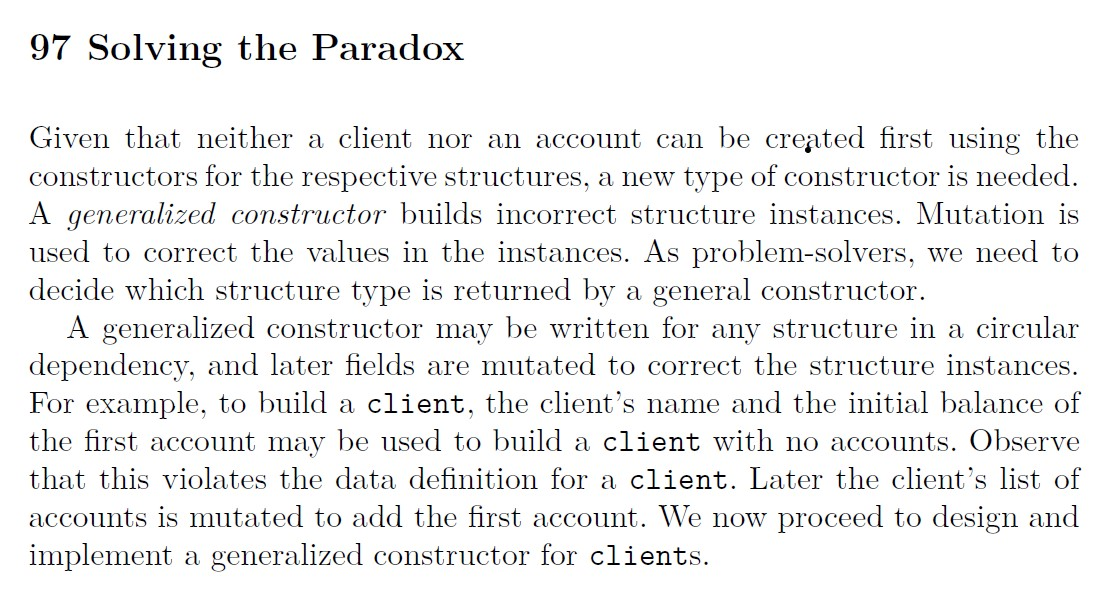
\includegraphics[scale=0.4]{generalized-constructor-APD.jpg}
\end{center}

\end{itemize}
\end{tiny}
\end{frame}

\begin{frame}[fragile]
\frametitle{Language Specification}
%\framesubtitle{HOMEWORK}
\begin{scriptsize}
\begin{itemize}
\item<1-> We need an env that contains a binding for all the local functions defined

\item<1->
$\frac{\rho_r = \texttt{[}n1=\texttt{(procedure p1 b1 }\rho_r)\texttt{]}\ldots \texttt{[}nn=\texttt{(procedure pn bn }\rho_r)\texttt{]}\rho}
      {(\text{value-of } (\text{letrec-exp (n1\ldots nn) (p1\ldots pn) (b1\ldots bn) body}) \ \rho) \ = \ (\text{value-of } body \ \rho_r)}$

\end{itemize}
\end{scriptsize}
\end{frame}

\section{Implementation}

\begin{frame}[fragile]
\frametitle{Implementation}
%\framesubtitle{HOMEWORK}
\begin{tiny}
\begin{itemize}
\item<1-> Procedure representation
\begin{alltt}
(define-datatype proc proc?
  (procedure
   (var (list-of symbol?))
   (body expression?)
   (envv voenv?)))
\end{alltt}

\item<2->
\begin{alltt}
;; Any \arrow{} Boolean
;; Purpose: Determine if given value is a vector with a single environment
(define (voenv? penv)
  (and (vector? penv)
       (= (vector-length penv) 1)
       (environment? (vector-ref penv 0))))
\end{alltt}


\end{itemize}
\end{tiny}
\end{frame}

\begin{frame}[fragile]
\frametitle{Implementation}
%\framesubtitle{HOMEWORK}
\begin{tiny}
\begin{itemize}
\item<1->
\begin{alltt}
;; value-of-program : program \arrow{} expval
;; Purpose: Evaluate the given program
(define (value-of-program pgm)
  (cases program pgm
    (a-program (exp1)
               (value-of exp1 (empty-env)))))
\end{alltt}

\item<2->
\begin{alltt}
;; value-of : expression env \arrow{} expval
;; Purpose: Evaluate the given expression in the given env
(define (value-of exp env)
  (cases expression exp
    (const-exp (num) \ldots)
    (true-exp () \ldots)
    (false-exp () \ldots)
    (var-exp (var) \ldots)
\end{alltt}

\item<3->
\begin{alltt}
    (diff-exp (exp1 exp2) \ldots (value-of exp1 env) (value-of exp2 env))
    (zero?-exp (exp1) \ldots (value-of exp1 env))
    (if-exp (exp1 exp2 exp3) \ldots
                             (value-of exp1 env)
                             (value-of exp2 env)
                             (value-of exp3 env))
\end{alltt}

\item<4->
\begin{alltt}
    (let-exp (vars exps body) \ldots
                              (map (lambda (e) (value-of e env)) exps)
                              (value-of body \dots))
\end{alltt}

\item<5->
\begin{alltt}
    (proc-exp (params body) \ldots)
    (call-exp (rator rands) \ldots
                            (value-of rator env)
                            (map (lambda (rand) (value-of rand env)) rands))
\end{alltt}

\item<6->
\begin{alltt}
    (letrec-exp (p-names params p-bodys letrec-body) (value-of letrec-body \ldots))))
\end{alltt}

\end{itemize}
\end{tiny}
\end{frame}

\begin{frame}[fragile]
\frametitle{Implementation}
%\framesubtitle{HOMEWORK}
\begin{scriptsize}
\begin{itemize}
\item<1-> Specializing \texttt{value-of}

\item<2->
\begin{alltt}
(const-exp (num) (num-val num))
\end{alltt}

\item<3-> (value-of (true-exp n) $\rho$) = (bool-val \#t)

\item<3-> (value-of (false-exp n) $\rho$) = (bool-val \#f)

\item<4->
\begin{alltt}
(var-exp (var) (apply-env env var))
\end{alltt}

\end{itemize}
\end{scriptsize}
\end{frame}

\begin{frame}[fragile]
\frametitle{Implementation}
%\framesubtitle{HOMEWORK}
\begin{scriptsize}
\begin{itemize}
\item<1->
$\frac{v1 = \text{(expval2num (value-of e1 } \rho)) \ \wedge \ v2 = \text{(expval2num (value-of e2 } \rho))}
      {\text{(diff-exp e1 e2) = (num-val (- v1 v2))}}$

\item<2->
\begin{alltt}
(diff-exp (exp1 exp2)
  (let ((num1 (expval2num (value-of exp1 env)))
        (num2 (expval2num (value-of exp2 env))))
    (num-val (- num1 num2))))
\end{alltt}

\item<3->
$\frac
{v = \text{(expval2num (value-of e)} \rho)}
{(\text{value-of (zero?-exp n) } \rho)=
 \begin{cases}
    \text{(bool-val \#t)}, & \text{if } v = 0\\
    \text{(bool-val \#f)}, & \text{if } v \neq 0\\
  \end{cases}}$

\item<4->
\begin{alltt}
(zero?-exp (exp1)
  (let ((val1 (expval2num (value-of exp1 env))))
    (if (zero? val1)
        (bool-val #t)
        (bool-val #f))))
\end{alltt}

\item<5->
$\frac
{cval = (\text{expval2bool } (\text{value-of } c \ \rho))}
{(\text{value-of } (\text{if-exp c t e} \rho) =
 \begin{cases}
   (\text{value-of } t \ \rho), & \text{if cval = \#t}\\
   (\text{value-of } e \ \rho), & \text{if cval = \#f}\\
 \end{cases}}$

\item<6->
\begin{alltt}
(if-exp (exp1 exp2 exp3)
  (let ((val1 (value-of exp1 env)))
    (if (expval2bool val1)
        (value-of exp2 env)
        (value-of exp3 env))))
\end{alltt}

\end{itemize}
\end{scriptsize}
\end{frame}

\begin{frame}[fragile]
\frametitle{Implementation}
%\framesubtitle{HOMEWORK}
\begin{scriptsize}
\begin{itemize}
\item<1->
$\frac{(v1\ldots vn) = (\text{map (lambda (e) (value-of e $\rho$))} (e1\dots en))}
      {(\text{value-of } (\text{let-exp (s1\ldots sn) (e1\ldots en) body}) \rho) \ = \ (\text{value-of } body \ [s1=v1\ldots sn=vn]\rho)}$

\item<2->
\begin{alltt}
(let-exp (vars exps body)
  (let [(vals (map (lambda (e) (value-of e env)) exps))]
    (value-of
      body
      (foldr (lambda (var val acc) (extend-env var val acc))
             env
             vars
             vals))))
\end{alltt}

\item<3-> (value-of (proc-exp (p1\dotss{}pn) b) $\rho$) = (proc-val (procedure (p1\dotss{}pn) b $\rho$))

\item<4->
\begin{alltt}
(proc-exp (params body)
  (proc-val (procedure params body (vector env))))
\end{alltt}

\item<5->
$\frac{p = (expval\texttt{->}proc (\texttt{value-of e0 } \rho)) \ \wedge{} \texttt{args = (map (lambda (e) (value-of e env)) }(e1\ldots{}en))}
      {\texttt{(value-of (call-exp e0 (e1} \ldots \texttt{en))} \rho) \texttt{ = (apply-procedure p args)}}$

\item<6->
\begin{alltt}
(call-exp (rator rands)
  (let [(proc (expval2proc (value-of rator env)))
        (args (map (lambda (rand) (value-of rand env)) rands))]
    (apply-procedure proc args)))
\end{alltt}

\end{itemize}
\end{scriptsize}
\end{frame}

\begin{frame}[fragile]
\frametitle{Implementation}
%\framesubtitle{HOMEWORK}
\begin{scriptsize}
\begin{itemize}
\item<1->
\begin{alltt}
;; apply-procedure : proc (listof expval) \arrow{} expval
;; Purpose: Apply the given procedure to the given values
(define (apply-procedure f vals)
  (cases proc f
    (procedure (params body envv)
      (let [(saved-env (vector-ref envv 0))]
        (value-of body
                  (foldr (lambda (binding acc)
                    (extend-env (car binding)
                                (cadr binding)
                                acc))
                    saved-env
                    (map (lambda (p v) (list p v))
                         params
                         vals)))))))
\end{alltt}
\end{itemize}
\end{scriptsize}
\end{frame}

\begin{frame}[fragile]
\frametitle{Implementation}
%\framesubtitle{HOMEWORK}
\begin{scriptsize}
\begin{itemize}
\item<1->
$\frac{\rho_r = \texttt{[}n1=\texttt{(procedure p1 b1 }\rho_r)\texttt{]}\ldots \texttt{[}nn=\texttt{(procedure pn bn }\rho_r)\texttt{]}\rho}
      {(\text{value-of } (\text{letrec-exp (n1\ldots nn) (p1\ldots pn) (b1\ldots bn) body}) \ \rho) \ = \ (\text{value-of } body \ \rho_r)}$

\item<2->
\begin{alltt}

;; (listof symbol) (listof (listof symbol)) (listof expression) env \arrow{} env
;; Purpose: Add proc-vals for given procedures in given environment
(define (mk-letrec-env ns ps bs env) \textcolor{darkgreen}{Generalized constructor}
  (let* [(temp-proc-vals
           (map (lambda (p b)           \textcolor{red}{Temporary wrong proc-vals}
                  (proc-val (procedure p b (vector (empty-env)))))
                ps
                bs))
\end{alltt}

\item<3->
\begin{alltt}
         (new-env (new-env (foldl (lambda (name proc env)
                                    (extend-env name proc env))
                           env
                           names
                           temp-proc-vals)))]
\end{alltt}

\item<4->
\begin{alltt}
    (begin
      (for-each (lambda (p)   \textcolor{darkgreen}{Correcting proc-vals}
                 (cases proc p
                  (procedure (p b ve) (vector-set! ve 0 new-env))))
                (map (lambda (p) (expval2proc p)) temp-proc-vals))
\end{alltt}

\item<5->
\begin{alltt}
      new-env)))
\end{alltt}

\end{itemize}
\end{scriptsize}
\end{frame}

\begin{frame}[fragile]
\frametitle{Implementation}
\framesubtitle{HOMEWORK}
\begin{scriptsize}
\begin{itemize}
\item<1-> Problems: 3.6--3.10, 3.12, 3.16--3.17, 3.21, 3.23--3.24, 3.26, 3.32--3.33, 3.55 (using the interpreter developed in class)
    
\item<1-> Some problems we have already solved!


\end{itemize}
\end{scriptsize}
\end{frame}


\section{Variable Names Elimination}

\begin{frame}[fragile]
\frametitle{Variable Names Elimination}
%\framesubtitle{HOMEWORK}
\begin{scriptsize}
\begin{itemize}
\item<1-> Several ways to declare vars: let, letrec, and proc (so far!)

\item<2-> In most PLs, declarations have limited scope
\begin{alltt}
(let [\textcolor{darkgreen}{(pi 3.14)}
	      \textcolor{darkgreen}{(e 2.71)}]
\fcolorbox{darkgreen}{white}{(+ (let [\textcolor{orange}{(pi 3.4)}]\newline
      \fcolorbox{orange}{white}{(+ pi e)})
    pi)})
\end{alltt}

\item<2-> Every programming language must have \emph{scoping rules}

\item<2-> Rules for determining the declaration for a variable reference

\item<3> In many PLs, search outward from the reference to the declaration

\item<3-> This is called lexical scoping and it is a static property

\end{itemize}
\end{scriptsize}
\end{frame}

\begin{frame}[fragile]
\frametitle{Variable Names Elimination}
%\framesubtitle{HOMEWORK}
\begin{scriptsize}
\begin{itemize}
\item<1->
\begin{alltt}
(let [\textcolor{darkgreen}{(pi 3.14)}
	      \textcolor{darkgreen}{(e 2.71)}]
\fcolorbox{darkgreen}{white}{(+ (let [\textcolor{orange}{(pi 3.4)}]
      \fcolorbox{orange}{white}{(+ \textcolor{orange}{pi} \textcolor{darkgreen}{e})})
    \textcolor{darkgreen}{pi})})
\end{alltt}

\item<1-> Holes in the scope of a var may be created by  nested declarations

\item<1-> The number of boxes crossed is the lexical depth of a var

\item<1-> The position in the declarations in the lexical position

\item<1-> Lexical address is both the lexical depth and lexical position

\item<2-> \textcolor{orange}{pi}: 0 0

\item<2-> e: 1 1

\item<2-> pi: 0 0

\item<3-> Why is this important?

\item<4-> Using lexical addresses eliminates the need to search for a binding in an environment.

\end{itemize}
\end{scriptsize}
\end{frame}

\begin{frame}[fragile]
\frametitle{Variable Names Elimination}
%\framesubtitle{HOMEWORK}
\begin{scriptsize}
\begin{itemize}
\item<1->
\begin{alltt}
(let [\textcolor{darkgreen}{(pi 3.14)}
	      \textcolor{darkgreen}{(e 2.71)}]
\fcolorbox{darkgreen}{white}{(+ (let [\textcolor{orange}{(pi 3.4)}]\newline
      \fcolorbox{orange}{white}{(+ \textcolor{orange}{pi} \textcolor{darkgreen}{e})})
    \textcolor{darkgreen}{pi})})
\end{alltt}

\item<2-> Implement an env as a list of ribs, where a rib is a list of expvals

\item<3->
\begin{center}
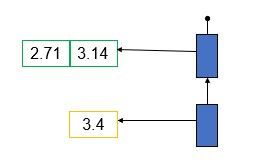
\includegraphics[scale=0.9]{nameless-env.jpg}
\end{center}

\item<4->
\begin{alltt}
(let [\textcolor{darkgreen}{(3.14 2.71)}]
\fcolorbox{darkgreen}{white}{(+ (let [\textcolor{orange}{(pi 3.4)}]\newline
      \fcolorbox{orange}{white}{(+ \textcolor{orange}{(0 0)} (1 1))})
    (0 0))})
\end{alltt}

\item<5-> The same is done for: proc, letrec

\item<5-> A variable becomes a lexical address

\item<5-> Add nameless versions for var, proc, let, and letrec to extended LC grammar

\item<5-> Change env representation

\end{itemize}
\end{scriptsize}
\end{frame}

\begin{frame}[fragile]
\frametitle{Variable Names Elimination}
%\framesubtitle{HOMEWORK}
\begin{scriptsize}
\begin{itemize}
\item<1->
\begin{alltt}
;;;;;    ENVIRONMENT

\#|

A rib is a (listof expval)

An environment is a (listof rib)

|\#
\end{alltt}

\item<2->
\begin{alltt}
(define (environment? e)
  (list-of (list-of expval?)))
\end{alltt}

\item<3->
\begin{alltt}
;;  \arrow{} environment
;; Purpose: Build the empty env
(define (empty-env) \elist{})
\end{alltt}

\item<4->
\begin{alltt}
;; (listof expval) environment \arrow{} environment
;; Purpose: Build an environment from given expvals and env
(define (extend-env vals env) (cons vals env))
\end{alltt}

\item<5->
\begin{alltt}
;; environment natnum natnum \arrow{} expval throws error
;; Purpose: Return expval at given lexical address in given env
(define (apply-env env depth pos)
  (if (empty? env)
      (eopl:error \quot{}apply-env "No binding for lexical address: ~s ~s" depth pos)
      (list-ref (list-ref env depth) pos)))
\end{alltt}

\end{itemize}
\end{scriptsize}
\end{frame}

\begin{frame}[fragile]
\frametitle{Variable Names Elimination}
%\framesubtitle{HOMEWORK}
\begin{scriptsize}
\begin{itemize}
\item<1-> New grammar rules

\item<1->
\begin{alltt}
(expression ("\%lexvar" number number) nameless-var-exp)

(expression ("\%nameless-proc" "(" expression ")") nameless-proc-exp)

(expression ("\%let" (arbno expression) "in" expression) nameless-let-exp)

(expression
  ("\%letrec" (arbno expression) "in" expression) nameless-letrec-exp)
\end{alltt}

\end{itemize}
\end{scriptsize}
\end{frame}

\begin{frame}[fragile]
\frametitle{Variable Names Elimination}
%\framesubtitle{HOMEWORK}
\begin{scriptsize}
\begin{itemize}
\item<1-> procs no longer need the store the parameter names
\begin{alltt}
(define-datatype proc proc?
  (procedure
   (body expression?)
   (envv voenv?)))
\end{alltt}

\item<2-> To evaluate we must translate a program to an equivalent nameless version
\begin{alltt}
;; string \arrow{} expval
;; Purpose: Evaluate the given extended LC-program
(define (eval string)
  (value-of-program (translate-program-nameless (parse string))))
\end{alltt}

\end{itemize}
\end{scriptsize}
\end{frame}

\begin{frame}[fragile]
\frametitle{Variable Names Elimination}
%\framesubtitle{HOMEWORK}
\begin{scriptsize}
\begin{itemize}
\item<1-> Refinements to value-of
\begin{alltt}
(nameless-var-exp (d p) (apply-env env d p))

(nameless-let-exp (exps body)
  (let [(vals (map (lambda (e) (value-of e env)) exps))]
    (value-of body (extend-env vals env))))

(nameless-proc-exp (body)
  (proc-val (procedure body (vector env))))

(nameless-letrec-exp (bodies letrec-body)
  (value-of letrec-body (mk-letrec-env bodies env)))
\end{alltt}

\end{itemize}
\end{scriptsize}
\end{frame}

\begin{frame}[fragile]
\frametitle{Variable Names Elimination}
\framesubtitle{HOMEWORK}
\begin{scriptsize}
\begin{itemize}
\item<1-> Problems: 3.38, 3.41 (using the interpreter developed in class)

\end{itemize}
\end{scriptsize}
\end{frame}

\end{document} 